\documentclass[../main.tex]{subfiles}
\usepackage{fancyhdr}
\graphicspath{{../images/}}

\begin{document}
\pagestyle{fancy}
\lhead{Physics 472: Li Yang}
\chead{Homework 6}
\rhead{Junseo Shin}

\renewcommand\thefigure{\arabic{figure}} 
\paragraph*{Problem 1.} (a) The displacement is given by
\begin{align*}
    x(t) &= \frac{1}{2\pi} \int_{-\infty}^\infty \alpha(\omega) e^{i \omega t} \dd{\omega}
\end{align*}
where the integral over the contour (the upper semicircle in the figure from Kittel) is zero since 
$\alpha(\omega)$ is
analytic in the uppper plane.
\begin{figure}[ht]
    \centering
    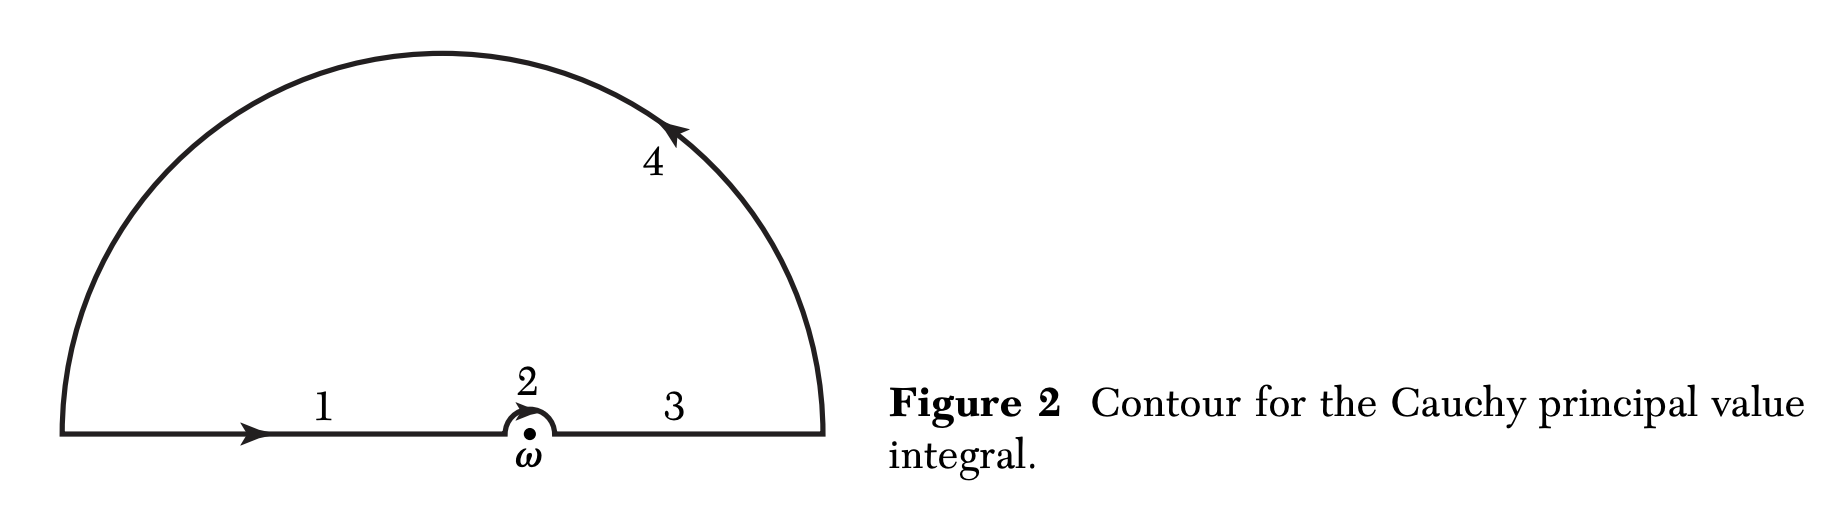
\includegraphics[width=0.8\linewidth]{cauchy.png}
\end{figure}
(b) 
\begin{align*}
    x(t) &= \frac{1}{2\pi} \int_{-\infty}^\infty \frac{ e^{i \omega t}}{\omega_0^2 - \omega^2 - i\omega \rho} \dd{\omega}
\end{align*}
Since the integral vanishes over the infinite semicircle, the Cauchy integral at the lower
half-plane, and with the residues at
\begin{align*}
    \pm \frac{1}{2} \qt(\omega_0^2 - \frac{1}{4} \rho^2)^{1/2} e^{-\rho t /2} e^{\mp i(\omega_0^2 - \frac{1}{4} \rho^2)^{1/2} t}
\end{align*}
the displacement is the imaginary part of the sum of the residues:
\begin{align*}
    x(t) = \qt(\omega_0^2 - \frac{1}{4} \rho^2)^{1/2} e^{-\rho t /2} \sin([\omega_0^2 - \frac{1}{4} \rho^2]^{1/2}t)
\end{align*}

\paragraph*{2} (a) Ferromagnetic Insulators:
\begin{itemize}
    \item EuO, Crystal Structure: SC, Curie Temp: 69 K (Kittel)
    \item EuS, Crystal Structure: SC, Curie Temp: 16 K (https://doi.org/10.1002/smll.200500294)
    \item CrBr$_3$, Crystal Structure: Hexagonal, Curie Temp: 37 K (https://doi.org/10.1016/j.physleta.2023.128980)
\end{itemize}
(b) Ferromagnetic Metals: (All from Kittel Ch 12 Table 1)
\begin{itemize}
    \item Fe, Crystal Structure: BCC, Curie Temp: 1043 K
    \item Co, Crystal Structure: HCP, Curie Temp: 1388 K
    \item Ni, Crystal Structure: FCC, Curie Temp: 627 K
\end{itemize}
(c) Antiferrromagnetic Insulators:
\begin{itemize}
    \item MnO, Crystal Structure: FCC, Neel Temp: 116 K (Kittel)
    \item MnS, Crystal Structure: FCC, Neel Temp: 160 K (Kittel)
    \item MnTe, Crystal Structure: Hexagonal, Neel Temp: 307 K (Kittel)
\end{itemize}
(d) Antiferromagnetic Metals:
\begin{itemize}
    \item Cr, CS: BCC, NT: 308 K (Kittel)
    \item VO$_2$, CS: Monoclinic, NT: 340 K(https://doi.org/10.1063/5.0027674)
    \item MnAs, CS: Hexagonal, NT: 480 K (DOI: 10.1103/PhysRevLett.111.047001)
\end{itemize}
\end{document}